\documentclass{scrartcl}
\usepackage[utf8]{inputenc}
\usepackage{hyperref}
\usepackage{url}
\usepackage[numbers]{natbib}
\usepackage{graphicx}
\usepackage{listings}
\usepackage{xcolor}
\usepackage{float}
\usepackage{tikz}
\usetikzlibrary{arrows.meta, positioning, calc, fit, backgrounds, shapes.geometric, shapes.multipart}
\usepackage{cleveref} % this must be the last package to be loaded

\lstset{
    basicstyle=\ttfamily\small,
    breaklines=true,
    frame=single,
    backgroundcolor=\color{gray!10}
}

\newcommand{\emailaddr}[1]{\href{mailto:#1}{\texttt{#1}}}

\title{\LARGE Distributed Bomberman}
\subtitle{Final Report for the Distributed Systems Course -- A.Y. 2024/25}

\author{
    Giovanni Rinchiuso \\ \emailaddr{giovanni.rinchiuso@studio.unibo.it}
    \and
    Gioele Santi \\ \emailaddr{gioele.santi2@studio.unibo.it}
}

\date{\today}

\begin{document}

\maketitle

\begin{abstract}
Distributed Bomberman is a real-time, fault-tolerant, multiplayer game inspired by the classic Bomberman arcade title, developed as a project for the Distributed Systems course at the University of Bologna (A.Y.\ 2024/25). Up to four players compete simultaneously on a shared grid, placing bombs to eliminate opponents. An unlimited number of spectators can observe the match and may request to join as a player when a slot becomes available. The system is built on an authoritative client-server architecture fronted by a session-aware TCP proxy, which hides a primary/backup server pair from clients. State is continuously replicated from the primary to the backup; on primary failure, the backup promotes itself automatically, re-binds the game port, and client sessions are restored transparently by the proxy; a second, independent retry loop on the client covers the failure of the proxy itself. The entire system is implemented in Python~3 using the standard library for networking and Pygame for the graphical client.
\end{abstract}

\newpage
\tableofcontents
\newpage

% -----------------------------------------------------------------------
\section{Concept}\label{concept}
% -----------------------------------------------------------------------

Distributed Bomberman is a system consisting of three cooperating processes: a game server, a transparent TCP proxy, and a Pygame graphical client.

\paragraph{Use cases.}
The main actors are the \textbf{Player}, the \textbf{Spectator}, and the \textbf{Host} (the first player to join, a special role assigned automatically).
Table~\ref{tab:usecases} summarises the principal use cases.

\begin{table}[h]
\centering
\small
\begin{tabular}{llp{6.5cm}}
\hline
\textbf{Use case} & \textbf{Actor} & \textbf{Description} \\
\hline
Join lobby & Player / Spectator & Connect, receive assigned name, enter lobby or spectator queue \\
Start game & Host & Press ``Start Game'' when $\geq 2$ players are connected \\
Move & Player & Send directional command; server updates position \\
Place bomb & Player & Place bomb at current tile; server handles detonation \\
Send chat & Player / Spectator & Broadcast a text message to all participants \\
Join as player & Spectator & Press J in the lobby; server converts spectator if a slot is free \\
Observe match & Spectator & Receive live state snapshots; no game interaction \\
\hline
\end{tabular}
\caption{Use cases of Distributed Bomberman.}
\label{tab:usecases}
\end{table}

\begin{figure}[h]
\centering
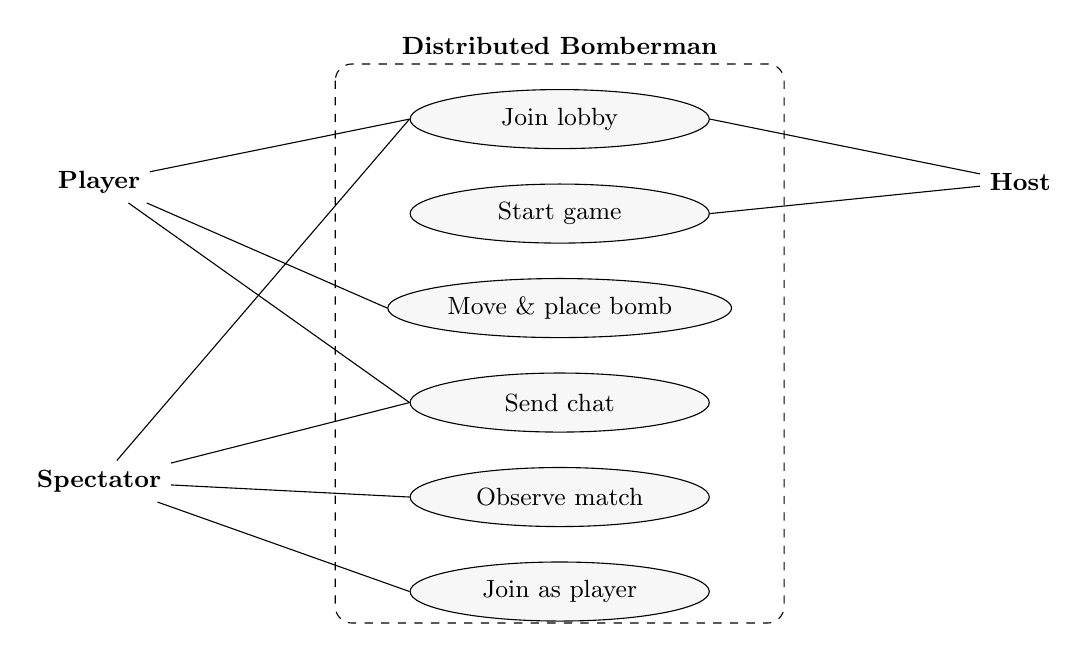
\begin{tikzpicture}[font=\small, >=Stealth,
  uc/.style  = {ellipse, draw, align=center, font=\small,
                minimum width=3.8cm, minimum height=0.75cm, fill=gray!6},
  act/.style = {font=\small\bfseries, align=center}
]
%% System boundary
\draw[rounded corners=6pt, dashed] (2.5,-0.5) rectangle (8.2,-7.6);
\node[font=\bfseries\small, above] at (5.35,-0.5) {Distributed Bomberman};

%% --- Actors ---
\node[act] (player)    at (-0.5,-2.0)  {Player};
\node[act] (spectator) at (-0.5,-5.8)  {Spectator};
\node[act] (host)      at (11.2,-2.0)  {Host};

%% --- Use cases (single column, even spacing) ---
\node[uc] (join)    at (5.35,-1.2) {Join lobby};
\node[uc] (start)   at (5.35,-2.4) {Start game};
\node[uc] (move)    at (5.35,-3.6) {Move \& place bomb};
\node[uc] (chat)    at (5.35,-4.8) {Send chat};
\node[uc] (observe) at (5.35,-6.0) {Observe match};
\node[uc] (joinp)   at (5.35,-7.2) {Join as player};

%% --- Player connections ---
\draw (player) -- (join.west);
\draw (player) -- (move.west);
\draw (player) -- (chat.west);

%% --- Spectator connections ---
\draw (spectator) -- (join.west);
\draw (spectator) -- (chat.west);
\draw (spectator) -- (observe.west);
\draw (spectator) -- (joinp.west);

%% --- Host connections ---
\draw (host) -- (join.east);
\draw (host) -- (start.east);
\end{tikzpicture}
\caption{Use case diagram of Distributed Bomberman.}
\label{fig:usecases}
\end{figure}

Players launch a client on their own machine; the client connects automatically to the proxy at a preconfigured address (default: \texttt{localhost:5555}) and is assigned a random name and a slot in the lobby.
Once at least two players have joined, the host can start the match.
Players move on a 2D grid, place bombs, and try to eliminate opponents; a player that runs out of lives is eliminated.
Spectators can join at any time and watch the match; while in the lobby, a spectator can request to become a player by pressing J, and is promoted if a slot is available.
The game ends when only one player remains alive (or all die simultaneously, resulting in a draw).
After a brief countdown, all players are returned to the lobby for a rematch.

\paragraph{Why distribution?}
Distribution is the core design driver:
\begin{itemize}
    \item \textbf{Multi-player real-time gameplay} requires clients on different machines to share a consistent, up-to-date view of the game state.
    \item \textbf{Authoritative server} centralises game logic, preventing clients from cheating and ensuring consistency.
    \item \textbf{Fault tolerance}: if the primary server crashes, a hot standby backup takes over automatically; clients experience a brief pause but do not need to reconnect manually.
\end{itemize}

\newpage
% -----------------------------------------------------------------------
\section{Requirements Identification and Analysis}\label{requirements}
% -----------------------------------------------------------------------

\subsection{Functional Requirements}

\begin{enumerate}
    \item[\textbf{F1}] Up to four players shall be able to join a shared lobby and play simultaneously on the same map.
    \item[\textbf{F2}] An unlimited number of spectators shall be able to join and observe the match in real time.
    \item[\textbf{F3}] While in the lobby, spectators shall be able to request to join as a player by pressing a dedicated key; the request is accepted if a player slot is currently available.
    \item[\textbf{F4}] The first player to join shall become the host and shall be able to start the game.
    \item[\textbf{F5}] Players shall be able to move on the grid and place bombs; bombs shall explode after a timer, destroying breakable blocks and damaging players in range.
    \item[\textbf{F6}] A player who disconnects during a match shall be marked as disconnected and excluded from the active game; their session can be restored under the original identity --- by the proxy after a server failover, or by the client itself once it re-establishes a dropped connection.
    \item[\textbf{F7}] Players shall be able to send chat messages visible to all participants.
    \item[\textbf{F8}] The system shall declare a winner (or a draw) and return all players to the lobby automatically.
\end{enumerate}

\subsection{Non-Functional Requirements}

\begin{enumerate}
    \item[\textbf{NF1}] \textbf{Fault tolerance}: the system shall continue operating if the primary server crashes; clients shall not need to manually reconnect.
    \item[\textbf{NF2}] \textbf{Consistency}: all clients shall observe the same game state; the server is the single source of truth.
    \item[\textbf{NF3}] \textbf{Latency}: the game loop shall tick every 100\,ms; the state broadcast interval shall not exceed 100\,ms.
    \item[\textbf{NF4}] \textbf{Transparency}: clients shall be unaware of the primary/backup topology; after a failover, the proxy shall restore all active client sessions to the new primary without requiring manual reconnection.
\end{enumerate}


\subsection{Relevant Distributed System Features}\label{ds-features}

\paragraph{Fault tolerance and dependability.}
The primary availability concern is that a server crash should not abort the ongoing match.
The system addresses this with a passive backup that receives state snapshots from the primary every 100\,ms and monitors it via heartbeat probes.
On failure detection (1.5\,s timeout), the backup promotes itself and rebinds the game port; the proxy then reconnects automatically.
The mechanism is straightforward and sufficient for the two-node, single-failure-domain scenario targeted by this project.

\paragraph{Transparency.}
Clients connect to a fixed proxy address and are unaware of the primary/backup topology (location and replication transparency).
During a failover, the proxy buffers incoming client data and flushes it once the new primary is reachable, making the switchover invisible to clients.
This is a limited form of failover transparency: it works well for short outages, but the proxy enforces a 30\,s timeout (\texttt{TCPProxy.FAILOVER\_TIMEOUT}) beyond which client connections are dropped.

\paragraph{Consistency.}
The authoritative server pattern provides a simple consistency model: only the server mutates game state, and clients are pure renderers.
All client inputs are serialised through the server's game loop under a single \texttt{RLock}, so there are no concurrent write conflicts.
One limitation worth noting is that the backup may hold a snapshot up to 100\,ms old at the time of failover, meaning a small amount of recent game state could be lost in a crash.

\paragraph{Performance and concurrency.}
The server uses one thread per client connection plus a dedicated game-loop thread.
State is broadcast to all clients every 100\,ms, which is adequate for a LAN setting with a small number of players.

\paragraph{Openness and evolvability.}
Communication uses TCP with line-delimited JSON, a deliberately simple protocol:
command verbs are dispatched by \texttt{CommandController} and the shared
parameters (ports, tick rate, map size) live in \texttt{src/common/constants.py}.
State snapshots carry a \texttt{"version"} field so that incompatible schema changes can be detected at runtime, and the three-process boundary means components can be updated independently within the constraints of the current protocol.

% -----------------------------------------------------------------------
\section{Design}\label{design}
% -----------------------------------------------------------------------

\subsection{Architecture}\label{architecture}

The system follows a \textbf{client-server} architectural style with a \textbf{proxy} interposed between clients and the server cluster.

The server cluster consists of a \textbf{primary} server and a single hot-standby \textbf{backup}, automatically respawned after each promotion.
The primary is the authoritative game engine; it replicates its state to the backup and exposes a heartbeat endpoint.
The backup monitors the primary and promotes itself on failure.
The proxy hides this topology from clients: it forwards traffic to a fixed backend port (the game port), buffers client data during failover, and reconnects to the new primary automatically.

This design was chosen because:
\begin{itemize}
    \item A centralised authoritative server simplifies consistency: there is a single source of truth.
    \item The proxy provides location transparency and simplifies client implementation.
    \item The primary/backup pattern provides fault tolerance without the complexity of consensus protocols, which is appropriate for a two-node cluster with a single failure domain.
\end{itemize}

\paragraph{Alternative architectures considered.}
The following alternatives were discarded in favour of the chosen design:

\begin{itemize}
    \item \textbf{Pure peer-to-peer}: Each client holds its own copy of the game state and propagates updates to peers.
    This avoids a single point of failure but introduces distributed consistency problems: concurrent inputs from multiple clients can easily produce diverging game states.
    Conflict resolution in a real-time game (e.g.\ two players moving to the same cell simultaneously) would require a consensus round for every input, adding unacceptable latency.

    \item \textbf{Direct client-to-server without proxy}: Clients connect directly to the primary.
    This would expose the primary's address to clients, making transparent failover impossible without requiring clients to implement their own discovery logic.
    The proxy layer is what enables location transparency and automatic reconnection.

    \item \textbf{Active-active replication (multi-master)}: Both primary and backup accept writes simultaneously.
    This would improve write availability but requires conflict resolution for concurrent game-state mutations, which is considerably more complex than the passive-backup approach and unjustified for a two-node cluster.
\end{itemize}

\begin{figure}[h]
\centering
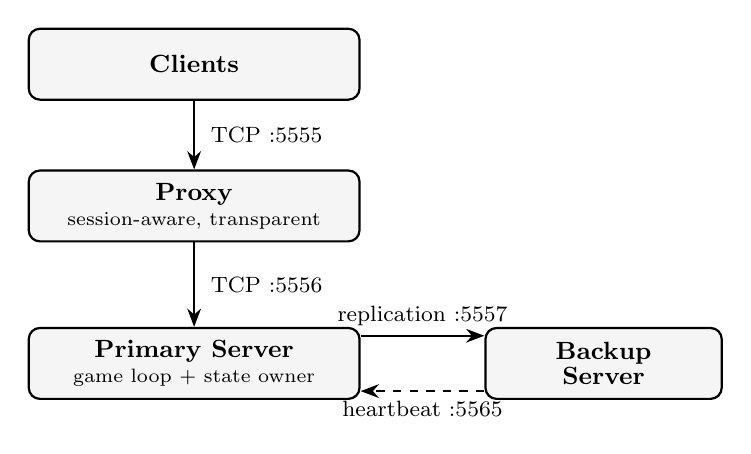
\begin{tikzpicture}[
  box/.style  = {draw, rounded corners=4pt, minimum width=4.2cm,
                 minimum height=0.9cm, align=center, fill=gray!8, font=\small},
  sbox/.style = {draw, rounded corners=4pt, minimum width=3.0cm,
                 minimum height=0.9cm, align=center, fill=gray!8, font=\small},
  >=Stealth, thick
]
  \node[box]  (C)  at (0,0)  {\textbf{Clients}};
  \node[box]  (Pr) at (0,-1.8)
      {\textbf{Proxy}\\[-2pt]\scriptsize session-aware, transparent};
  \node[box]  (Prim) at (0,-3.8)
      {\textbf{Primary Server}\\[-2pt]\scriptsize game loop + state owner};
  \node[sbox] (B)  at (5.2,-3.8)
      {\textbf{Backup}\\[-2pt]\textbf{Server}};

  \draw[->] (C)   -- node[right, font=\footnotesize]{\;TCP :5555} (Pr);
  \draw[->] (Pr)  -- node[right, font=\footnotesize]{\;TCP :5556} (Prim);
  \draw[->] ([yshift=10pt]Prim.east) --
            node[above, font=\footnotesize]{replication :5557}
            ([yshift=10pt]B.west);
  \draw[->, dashed] ([yshift=-10pt]B.west) --
            node[below, font=\footnotesize]{heartbeat :5565}
            ([yshift=-10pt]Prim.east);
\end{tikzpicture}
\caption{High-level architecture of Distributed Bomberman.}
\label{fig:architecture}
\end{figure}

\subsection{Infrastructure}\label{infrastructure}

\paragraph{Infrastructural components.}
Three process types are required to run the system; all can run on the same machine or on separate machines on the same LAN:

\begin{itemize}
    \item \textbf{Server cluster} ($1 + 1$ instances): one active \emph{primary} server (port~5556) and one \emph{backup} server, which uses two ports: 5557 for receiving state snapshots (\texttt{BACKUP\_STATE\_PORT}) and 5558 as its own game port before promotion (\texttt{BACKUP\_GAME\_PORT}). Only the primary hosts the live \texttt{GameService} and accepts client connections; the backup runs in passive monitoring mode, receiving periodic state snapshots and waiting to be promoted. The primary automatically spawns the backup at startup via the \texttt{AutoSpawner} component; each newly promoted backup spawns a new one, maintaining fault tolerance continuously.

    \item \textbf{TCP proxy} (port 5555): a transparent relay that hides the primary/backup topology from clients. It forwards data in both directions, captures per-client \texttt{session\_id}s from the server's join acknowledgements, and manages failover transparently by buffering client data and sending \texttt{RECONNECT} handshakes to the new primary.

    \item \textbf{Client nodes} ($N$ instances): Pygame graphical client applications that connect to the proxy at a pre-configured address. Each client is a pure renderer: it sends input commands and renders whatever state snapshot the server broadcasts.
\end{itemize}

\paragraph{Network distribution.}
All components communicate over standard TCP/IP sockets on a local area network.

\paragraph{Service discovery.}
Components locate each other through \textbf{static port configuration} defined in \texttt{src/common/constants.py}.
This is a deliberate design choice justified by the deployment scenario:
\begin{itemize}
    \item The server cluster is a fixed two-node setup (primary + backup); there is no need to discover a dynamically changing set of server nodes.
    \item Clients always connect through the proxy at a single, well-known address; if the proxy address changes, clients simply update the one constant.
    \item A dynamic discovery mechanism (e.g.\ UDP broadcast) would add complexity without benefit for a LAN-local system with a fixed topology.
\end{itemize}

\subsection{Modelling}\label{modelling}

\paragraph{Domain entities.}
The key domain entities are:
\begin{itemize}
    \item \textbf{Player}: position $(x, y)$, name, lives, alive/disconnected status, reconnect session ID.
    \item \textbf{Spectator}: name, join time, connected status.
    \item \textbf{Bomb}: position, countdown timer, owner player ID.
    \item \textbf{Explosion}: set of affected tiles, remaining display ticks.
    \item \textbf{State}: the complete, versioned snapshot of the game -- game phase (\texttt{lobby / playing / victory}), map, all players, spectators, bombs, explosions, chat messages, winner.
\end{itemize}


\paragraph{Domain class diagram.}
Figure~\ref{fig:classes} shows the key domain classes and their relationships. Secondary entities (\texttt{Explosion}, \texttt{Spectator}) are omitted from the diagram for clarity but are part of the \texttt{State} snapshot.

\begin{figure}[H]
    \centering
    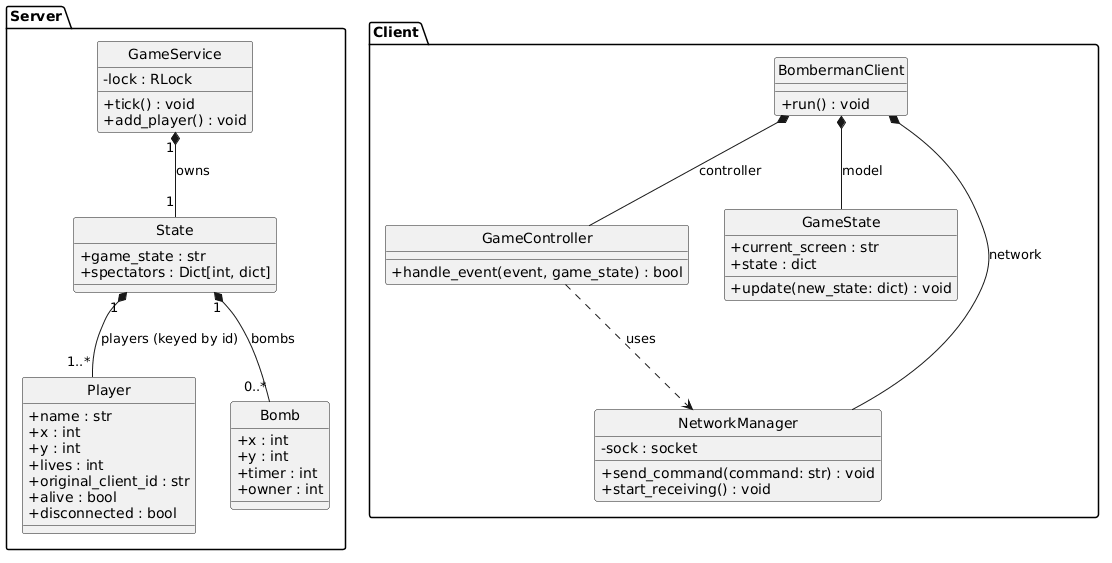
\includegraphics[width=0.8\textwidth]{figures/UMLUno.png}
    \caption{Domain class diagram of Distributed Bomberman.}
    \label{fig:classes}
\end{figure}

\paragraph{Component overview.}
Figure~\ref{fig:components} shows the main components of the four processes and the channels connecting them.

\begin{figure}[H]
    \centering
    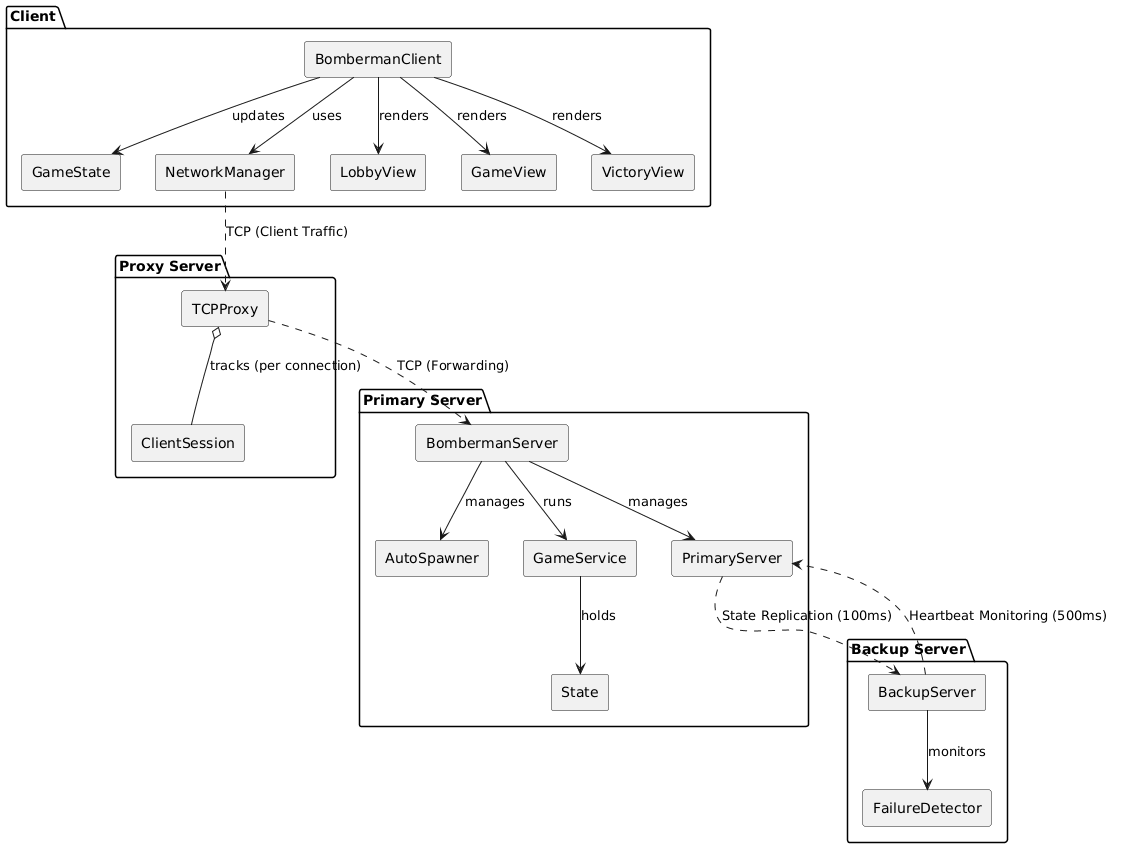
\includegraphics[width=0.95\textwidth]{figures/UMLDue.png}
    \caption{Component overview of Distributed Bomberman.}
    \label{fig:components}
\end{figure}

\paragraph{State ownership.}
The \texttt{State} object lives exclusively on the server.
Clients receive a serialised projection of the state at each tick; they never mutate it directly.

Two distinct serialisations are used. Clients receive a \emph{phase-dependent
projection} produced by \texttt{GameService.get\_state()}: it always carries the
game phase, players, spectators, chat and host, and adds only the fields relevant
to the current phase --- lobby eligibility flags in \texttt{lobby}, the map, bombs
and explosions in \texttt{playing}, the winner and countdown in \texttt{victory}.
Replication to the backup instead uses the full versioned codec
(\texttt{state\_to\_dict} / \texttt{state\_from\_dict}), which serialises every
field without exception: the backup must be able to resume the match from that
snapshot alone, so a partial projection would be insufficient.

\paragraph{Messages.}
Three classes of messages are exchanged:
\begin{itemize}
    \item \textbf{Commands} (client $\to$ server): \texttt{UP}, \texttt{DOWN},
    \texttt{LEFT}, \texttt{RIGHT} (movement), \texttt{BOMB},
    \texttt{START\_GAME}, \texttt{PLAY\_AGAIN}, \texttt{JOIN\_GAME} (spectator
    requests a player slot), \texttt{CHAT:\{message\}}. The server also accepts
    a \texttt{PING} command for manual connectivity checks (e.g.\ over
    \texttt{netcat}); the graphical client never sends it.
    Commands are case-insensitive and newline-terminated.
    \item \textbf{State snapshots} (server $\to$ client): the JSON projection of
    the current state described above, sent every 100\,ms.    \item \textbf{Control messages}: \texttt{RECONNECT:\{session\_id\}} (sent to the server by the proxy after a failover, or by the client after it re-establishes a dropped connection), \texttt{HEARTBEAT} / \texttt{ALIVE} (backup $\leftrightarrow$ primary).
\end{itemize}

\subsection{Interaction}\label{interaction}

\paragraph{Interaction pattern.}
Distributed Bomberman uses a \textbf{pure client-server} interaction model: all communication — game commands, state updates, chat — flows through the proxy to the primary server.

This choice was deliberate:
\begin{itemize}
    \item \textbf{Consistency}: a single serialisation point (the server game loop) eliminates the possibility of concurrent writes and distributed state divergence.
    \item \textbf{Simplicity}: clients have no peer-discovery logic, no direct connections to other clients, and no need to synchronise local replicas.
    \item \textbf{Fault tolerance}: the proxy-mediated model makes failover transparent; clients never know which physical server they are talking to.
\end{itemize}
The trade-off is that the server becomes a bandwidth bottleneck for state broadcasts, which is acceptable given the small player count (max 4) and the 100\,ms tick rate.

\paragraph{Communication model.}
All messages are serialised as \textbf{line-delimited JSON} over persistent TCP connections (one connection per client, kept open for the entire session).
The server operates in a \textbf{publish-subscribe} style for state updates: after each game tick it pushes a state snapshot to all connected clients simultaneously, without waiting for a request.
Client-to-server commands follow a \textbf{fire-and-forget} pattern: the client sends a command (e.g.\ \texttt{UP}) and immediately continues; the effect appears in the next state broadcast.

\paragraph{Join sequence.}
Figure~\ref{fig:seq-join} shows the message flow when a client connects.

\begin{figure}[H]
    \centering
    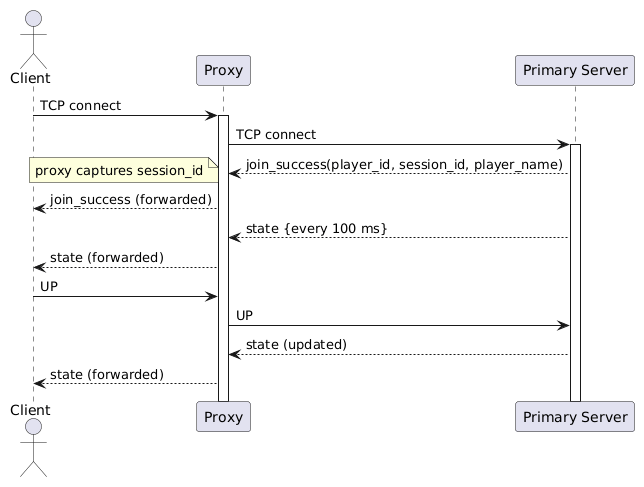
\includegraphics[width=0.7\textwidth]{figures/UMLTre.png}
    \caption{Join and normal operation sequence diagram.}
    \label{fig:seq-join}
\end{figure}

On join, the server sends a \texttt{join\_success} JSON object containing the player's assigned ID and a unique \texttt{session\_id} (UUID4).
The proxy captures this session ID and uses it to send a \texttt{RECONNECT:\{session\_id\}} message to the new primary after a failover.

\paragraph{Game-start sequence.}
Figure~\ref{fig:seq-start} shows the message flow when the host starts the match.

\begin{figure}[H]
    \centering
    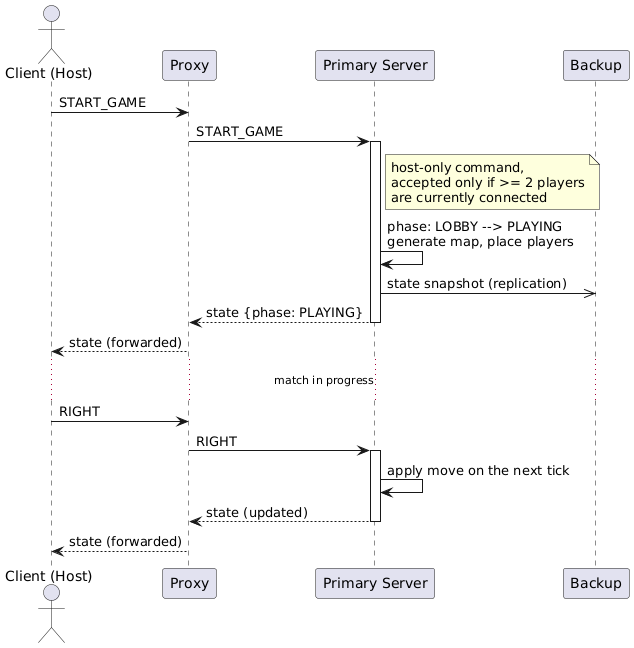
\includegraphics[width=0.85\textwidth]{figures/game_start.png}
    \caption{Game-start sequence diagram.}
    \label{fig:seq-start}
\end{figure}

\paragraph{Failover sequence.}
Figure~\ref{fig:seq-failover} shows the message flow during a primary server failure and recovery.

\begin{figure}[H]
    \centering
    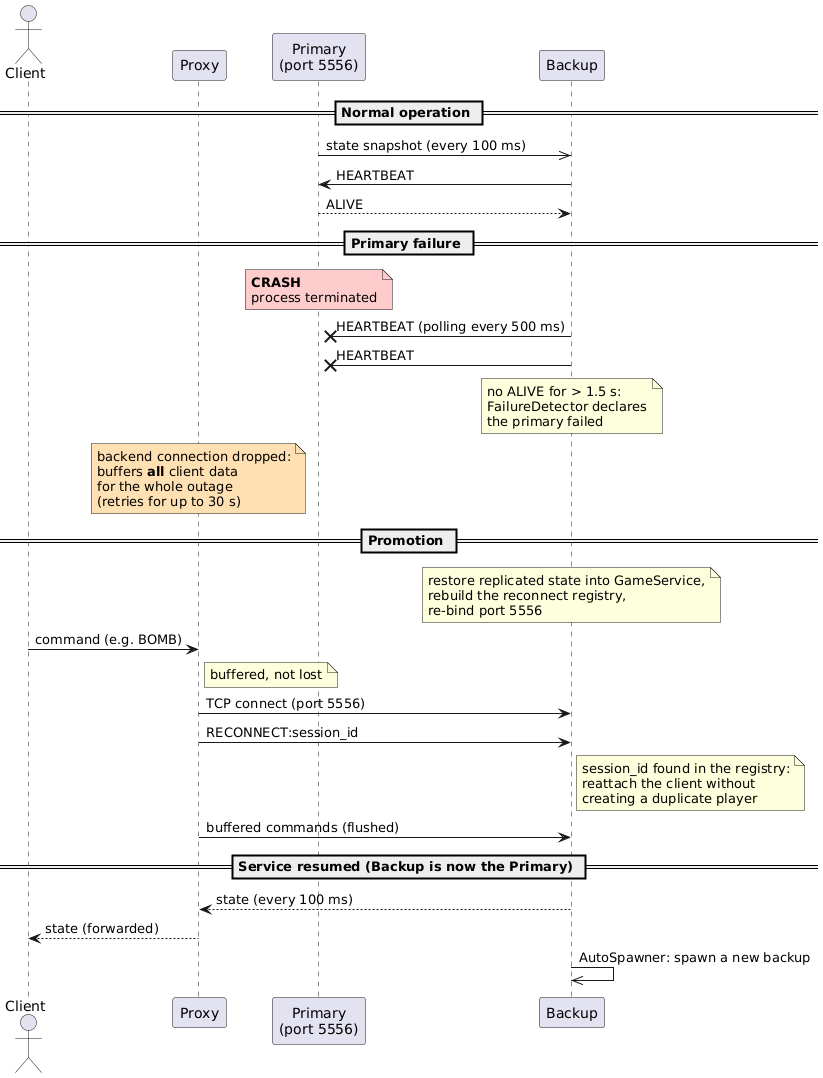
\includegraphics[width=0.6\textwidth]{figures/failover.png}
    \caption{Failover sequence diagram.}
    \label{fig:seq-failover}
\end{figure}

Primary-to-backup replication uses a separate TCP connection per snapshot: the primary opens a fresh connection to the backup's state-receiver port, sends a length-prefixed JSON payload, and closes it. This approach is simple to implement but creates a new connection every 100\,ms; a persistent replication channel would be more efficient, though the overhead is negligible at this scale.

\subsection{Behaviour}\label{behaviour}

\paragraph{Game phase state machine.}
The server \texttt{State} object progresses through three distinct phases (Figure~\ref{fig:fsm}):

\begin{figure}[h]
\centering
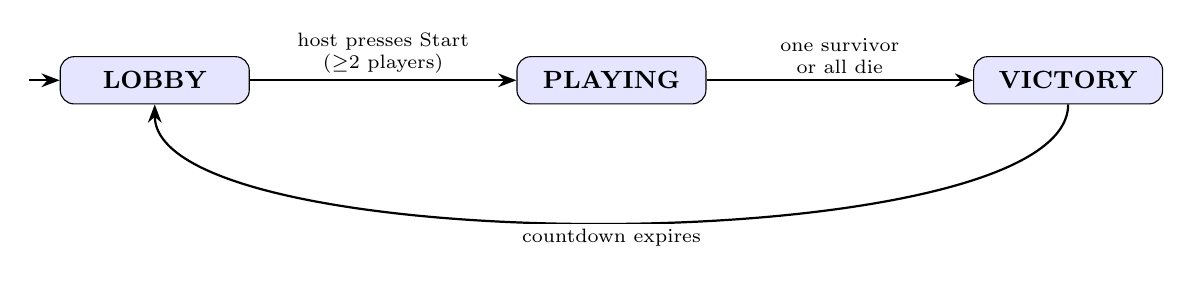
\begin{tikzpicture}[font=\small, >=Stealth,
  state/.style = {draw, rounded corners=5pt, minimum width=2.4cm,
                  minimum height=0.6cm, align=center,
                  fill=blue!10, font=\bfseries\small},
  lbl/.style   = {font=\scriptsize, align=center, fill=white, inner sep=2pt}
]
  \node[state] (L) at (0,0)    {LOBBY};
  \node[state] (P) at (5.8,0)  {PLAYING};
  \node[state] (V) at (11.6,0) {VICTORY};

  %% initial arrow
  \draw[->, thick] (-1.6,0) -- (L);

  %% LOBBY -> PLAYING
  \draw[->, thick] (L) -- node[lbl, above]{host presses Start\\($\geq$2 players)} (P);

  %% PLAYING -> VICTORY
  \draw[->, thick] (P) -- node[lbl, above]{one survivor\\or all die} (V);

  %% VICTORY -> LOBBY (arc below)
  \draw[->, thick] (V.south) .. controls +(0,-2.0) and +(0,-2.0) ..
      node[lbl, below]{countdown expires} (L.south);
\end{tikzpicture}
\caption{Server game phase state machine.}
\label{fig:fsm}
\end{figure}

\textbf{LOBBY}: The server waits for players to connect.
The host can start the game when at least two players are present.
Spectators may request a player slot by pressing J (lobby only; not permitted during an active match).
A player who disconnects in the lobby is removed immediately.

\textbf{PLAYING}: The game loop is active.
Players move and place bombs; the server processes inputs, detonates bombs, computes explosions, and reduces player lives.
A player who disconnects mid-game is marked \texttt{disconnected=True, alive=False}, and the disconnection immediately triggers a victory check.
Session restoration via the \texttt{RECONNECT} handshake is triggered either by the
proxy after a primary failover, or by the client itself after it re-establishes a
dropped connection --- provided the client process stayed alive and still holds its
\texttt{session\_id}.
Reattaching therefore restores the player's identity and clears the disconnected
flag, but it does not undo a phase transition that the victory check has already
performed.

\textbf{VICTORY}: One player has survived (or all died simultaneously for a draw).
The winner is recorded.
A countdown runs (the ``return to lobby'' timer); when it expires, the state is reset to LOBBY and a new match can begin.

\paragraph{Game loop (server).}
The server runs a fixed-rate game loop at 10\,Hz (100\,ms per tick).
Each tick:
\begin{enumerate}
    \item Decrement bomb timers; detonate expired bombs, compute explosion cells, reduce player lives.
    \item Decrement explosion display timers; remove expired explosions.
    \item Check victory conditions.
    \item If in the victory phase, decrement the return-to-lobby timer.
    \item Broadcast the current state projection to all connected clients and spectators.
\end{enumerate}

\paragraph{Client reactive behaviour.}
The client does not implement its own state machine.
Instead it behaves as a \textbf{reactive consumer}: it renders whatever state the server broadcasts.
The \texttt{GameState} model inspects the \texttt{game\_state} field of each received snapshot and updates \texttt{current\_screen} accordingly; the main loop then switches the active view:
\begin{itemize}
  \item \texttt{lobby} $\Rightarrow$ \texttt{LobbyView}: displays connected players, spectators, and the ``Start Game'' button (host only).
  \item \texttt{playing} $\Rightarrow$ \texttt{GameView}: renders the grid, players, bombs, and explosions in real time.
  \item \texttt{victory} $\Rightarrow$ \texttt{VictoryView}: shows the winner (or draw) and the return-to-lobby countdown.
\end{itemize}
This design keeps failover handling minimal on the client: when the proxy restores the TCP stream, the next state broadcast simply resumes rendering, and no view is aware that a switchover occurred.
The client is not entirely passive, however --- it owns the recovery path for a failure of the proxy itself, described in \cref{availability}.

\subsection{Data and Consistency Issues}\label{data-and-consistency-issues}

No persistent storage is used: all game state is in memory.
State is only replicated between the primary and the backup for fault tolerance purposes, not for durability.
On a complete cluster failure (both primary and backup crash simultaneously), the game state is lost.

Concurrent access to the \texttt{GameService} is serialised through a single \texttt{threading.RLock}, ensuring that client handler threads and the game loop thread never mutate the state concurrently.

\paragraph{Consistency model.}
From the clients' perspective, the system provides a straightforward consistency model: every state snapshot broadcast by the server reflects all inputs processed up to that tick, and clients never modify state locally.
In practice, clients observe state that is at most one tick old (100\,ms), which is acceptable for the target use case.

Between the primary and the backup, consistency is \textbf{eventual} rather than strong: the backup's replicated state lags the primary by at most one replication interval (100\,ms).
This means that in the event of a primary crash, the backup may be missing up to 100\,ms of game events.
This trade-off was intentional: synchronous replication (waiting for a backup acknowledgement before processing each input) would have added per-tick latency unacceptable for a real-time game.

\paragraph{State versioning.}
Each snapshot sent to the backup includes a \texttt{"version"} field (currently \texttt{1}).
The backup checks this field on receipt and discards snapshots with an incompatible version.
This prevents a stale or malformed snapshot from corrupting the backup's state after a code upgrade.

\paragraph{Replication completeness.}
The state codec (\texttt{state\_to\_dict} / \texttt{state\_from\_dict}) serialises the complete game state, including all player fields (position, lives, session IDs, disconnection status), all active bombs and explosions, spectator list, chat history, and game phase.
The serialisation round-trip is verified by a dedicated test module (\texttt{test\_state\_codec.py}) to ensure that no field is silently dropped or corrupted during replication.

\subsection{Fault-Tolerance}\label{fault-tolerance}

\paragraph{State replication.}
The primary serialises the full \texttt{State} as a versioned JSON snapshot and pushes it to the backup every 100\,ms.
The backup deserialises the snapshot and keeps it in memory as \texttt{replicated\_state}.
On promotion, the backup restores this state directly into its \texttt{GameService}.

\paragraph{Failure detection.}
The \texttt{FailureDetector} class tracks the timestamp of the last successful heartbeat.
It declares the primary failed if no heartbeat has been received for more than 1.5\,s.
The backup polls the primary's heartbeat port (TCP, short-lived connections) every 500\,ms.

\paragraph{Post-failover session restore.}
When a player disconnects, the server removes the entry outright if the game is in
the lobby; during a running match it keeps the entry and marks it
\texttt{disconnected=True, alive=False}, so that there is still something to
reattach to later.

The \texttt{RECONNECT} handshake has two senders. After a primary failover the
proxy sends the \texttt{session\_id} it captured from the original
\texttt{join\_success}; after a dropped connection the client sends the
\texttt{session\_id} it stored itself. In both cases the primary looks it up in the
reconnect registry --- rebuilt from the replicated state after a promotion --- and
re-attaches the client without creating a duplicate player entry, clearing the
disconnected flag and restoring the player to active play. The restore is
deliberately conservative: it acts only on a player marked \texttt{disconnected}, so
a player eliminated in combat is never resurrected by reconnecting.

\paragraph{Proxy buffering.}
During failover the proxy keeps client-side TCP connections open and accumulates
everything the client sends. Crucially, the reconnection retry loop polls the
client socket non-blockingly on every attempt. An earlier implementation blocked
inside the retry wait, which also stalled the relay loop: the client socket was
never read for the duration of the outage, so only the chunk in flight at the
moment of detection was ever captured, and every command issued during the outage
was lost. Once the new primary accepts the connection, the
\texttt{RECONNECT} handshake is sent and the accumulated buffer is flushed before
normal forwarding resumes.

\subsection{Availability}\label{availability}

The proxy acts as a single logical entry point.
It does not perform load balancing (there is only one active server at any time) but it hides the primary/backup switchover from clients, so that service continues across a primary crash.

There is no caching layer: clients always receive a fresh state broadcast every 100\,ms.

\paragraph{CAP theorem analysis.}
In the CAP theorem framework, a distributed system can guarantee at most two of
\textbf{Consistency}, \textbf{Availability}, and \textbf{Partition tolerance}.
Partition tolerance is not an optional property in any real network --- partitions
can always occur --- so the meaningful question is how the system behaves
\emph{when} one happens.

In the absence of partitions, Distributed Bomberman provides both consistency and
availability: all clients observe the same game state, since the authoritative
server is the single source of truth and clients never mutate state locally, and
the primary/backup pair combined with proxy buffering keeps the service running
across a primary crash.

Under a partition, however, the system favours \textbf{availability} over
consistency. The backup promotes itself unilaterally as soon as the heartbeat
times out (1.5\,s), with no quorum and no fencing mechanism to demote the old
primary. If a partition separates primary and backup while both processes remain
alive, both can act as primary simultaneously --- a \textbf{split-brain} --- and
their states diverge with no reconciliation once the partition heals. The system
therefore does \emph{not} guarantee consistency under partition: in CAP terms it
is \textbf{AP}-leaning. Making it genuinely CP would require replacing the
timeout-based promotion with a quorum-based leader election over an odd number of
nodes, for example Raft, together with a fencing token
ensuring that a demoted primary cannot continue to serve clients. This was judged
disproportionate for a two-node cluster in a single failure domain, but it is the
principal correctness limitation of the current design.

A second structural limitation is that the proxy is a \textbf{single point of
failure} for availability: while it is down no client can reach the cluster, even
though both servers are healthy. Its impact is partly bounded by a second and
independent recovery layer implemented on the client: when the connection drops
the client retries the proxy address every two seconds and, once the proxy is
reachable again, replays the \texttt{RECONNECT:\{session\_id\}} handshake itself,
so the primary reattaches the existing player instead of creating a new one.

The two layers are not equivalent, however, and the asymmetry is instructive. A
primary crash is invisible to clients precisely because the dying primary never
observes the disconnection: the backup resumes from a snapshot in which every
player is still alive. A proxy crash is different, because the primary stays alive
and does observe every client socket closing. Each disconnection marks the player
\texttt{disconnected} and \texttt{alive=False} and triggers a victory check, so in
a two-player match the first drop already ends the round. The client's retry loop
therefore preserves the \emph{session} --- players reattach under their original
identity rather than rejoining as new ones --- but it does not preserve an
\emph{in-progress match}. Making proxy failure fully transparent would require the
primary to distinguish a transport failure from a player quitting, for instance by
suspending the victory check for a grace period after a disconnection instead of
evaluating it immediately.

% -----------------------------------------------------------------------
\section{Implementation}\label{implementation}
% -----------------------------------------------------------------------

\subsection{Technology Stack}

The system is implemented in \textbf{Python 3.10+}, using only the standard library for networking (\texttt{socket}, \texttt{threading}, \texttt{json}).
The graphical client is built with \textbf{Pygame 2.5}, chosen for its suitability for real-time 2D rendering and its straightforward event loop.
Inter-component communication uses \textbf{JSON over TCP}, a deliberate choice over binary formats for human-readability and ease of debugging.
The project is packaged with \textbf{Poetry}  for reproducible dependency management, with entry points \texttt{bomberman-server}, \texttt{bomberman-proxy}, and \texttt{bomberman-client}.
The test suite is written with Python's \textbf{unittest} framework and run with \textbf{pytest}.
Session IDs are generated using \textbf{UUID4} from the standard library.

\paragraph{Network protocol.}
All communication uses \textbf{TCP} (Python \texttt{socket} module).
TCP was chosen over UDP because the game uses an authoritative server model: every client input must be delivered reliably and in order.

\paragraph{Message framing.}
TCP is a byte stream, not a message stream: a single \texttt{recv()} may return
several concatenated commands, or only part of one. All application messages are
therefore newline-delimited, and both endpoints accumulate incoming bytes in a
buffer which is split on \texttt{\textbackslash n} rather than being treated as
one message per \texttt{recv()}. The buffer is capped at 64\,KB, so that a peer
which never terminates a frame has its connection dropped instead of growing the
buffer without bound.

Framing interacts directly with failover. When the proxy reconnects to the newly
promoted primary it writes the \texttt{RECONNECT:\{session\_id\}} handshake
immediately followed by every command buffered during the outage, frequently
within the same TCP segment. The server therefore preserves whatever follows the
handshake line and uses it to seed the client handler's framing buffer, so that
commands issued while the primary was down are executed rather than silently
discarded.

\paragraph{Data representation.}
All messages are serialised as \textbf{JSON}, one object per line (\texttt{{\textbackslash}n}-delimited).
JSON was chosen for its human-readability (useful for debugging) and for native Python support via the \texttt{json} standard library module.
The state snapshot uses a versioned schema (\texttt{"version": 1}) to detect incompatible snapshots during replication.

\paragraph{Concurrency model.}
The server uses \textbf{one thread per client connection} plus a dedicated game-loop thread and fault-tolerance threads (heartbeat responder, replication sender).
Access to the shared \texttt{GameService} is protected by a single \texttt{threading.RLock}.

\paragraph{MVC on the client.}
The client is structured following the \textbf{Model-View-Controller} pattern:
\begin{itemize}
    \item \textbf{Model} (\texttt{GameState}): holds the last received state snapshot.
    \item \textbf{View} (\texttt{LobbyView}, \texttt{GameView}, \texttt{VictoryView}, \ldots): renders the current screen using Pygame.
    \item \textbf{Controller} (\texttt{GameController}): translates keyboard input into server commands.
    \item \textbf{Network} (\texttt{NetworkManager}): handles the TCP connection and message framing in a background thread.
\end{itemize}

The MVC separation means that the client's rendering logic is completely decoupled from the network layer.
When the \texttt{NetworkManager} thread receives a new state snapshot, it updates the \texttt{GameState} model; the Pygame main loop then re-renders whatever the model currently holds.
This design also simplifies the failover scenario on the client side: since the client has no concept of ``which server'' it is connected to, a reconnection requires no change to the model, the views or the controller.
Only the transport is replaced --- \texttt{BombermanClient.reconnect()} swaps in a fresh \texttt{NetworkManager}, carries the previous \texttt{session\_id} over to it and replays the \texttt{RECONNECT} handshake, leaving the Pygame window and the rendering loop untouched.

\paragraph{Proxy implementation.}
The proxy spawns one thread per client connection.
Each thread manages both directions of the relay — client-to-backend and backend-to-client — using \texttt{select()} to multiplex the two sockets without blocking.
During failover, the thread detects the backend drop, accumulates incoming client data in a local buffer (\texttt{client\_buf}), and retries the backend connection for up to 30\,s.
Once reconnected, it sends the \texttt{RECONNECT:\{session\_id\}} handshake and flushes the buffer before resuming normal forwarding.

\paragraph{AutoSpawner and process management.}
The \texttt{AutoSpawner} uses Python's \texttt{subprocess} module to launch the backup server as a child process.
When the backup is promoted to primary, it invokes \texttt{AutoSpawner} again to spawn a new backup, maintaining fault tolerance continuously.
If the backup process terminates unexpectedly, a background monitor thread detects the failure and automatically respawns a new backup, so the replication channel is restored without operator intervention.


% -----------------------------------------------------------------------
\section{Validation}\label{validation}
% -----------------------------------------------------------------------

\subsection{Automatic Testing}\label{automatic-testing}

Validation was performed through a combination of automated unit testing and manual end-to-end testing.
The automated test suite consists of 100 tests across five modules, located in \texttt{src/test/} and executable with:
\begin{lstlisting}
poetry run pytest src/test
\end{lstlisting}
Tests use Python's \texttt{unittest} framework. Where network or Pygame dependencies would be required, components are isolated using \texttt{unittest.mock} (\texttt{Mock}, \texttt{patch}), allowing each layer to be tested independently.

\paragraph{test\_core.py -- 18 unit tests for pure game logic.}
Tests cover: safe zone computation, player spawn points, connected player count, spectator join eligibility, chat message handling, map generation (boundary walls, safe spawn areas), tile walkability, player presence checks, movement, bomb placement and explosion propagation, victory detection (single winner and draw), block regeneration safety, and lobby reset.
All tests are deterministic and require no network or Pygame initialisation.

One test is a regression test for spectator-slot eligibility with a disconnected
player: that branch referenced a field which had been removed from the
\texttt{Player} dataclass, and since no existing test exercised it the resulting
\texttt{AttributeError} --- reachable from inside the game loop --- went unnoticed
until a manual code review.

\paragraph{test\_game.py -- 31 client-side unit tests.}
Tests cover the \texttt{GameState} model (initial state, phase transitions on lobby/playing/victory snapshots, player and spectator data extraction) and the \texttt{GameController} (key bindings for movement, bomb placement, chat activation, spectator join request, host start command).
Network dependencies are replaced with \texttt{Mock} objects, isolating the controller from the TCP layer.

\paragraph{test\_controller.py -- 28 command and network unit tests.}
Tests cover the server-side \texttt{CommandController} (movement, bomb, game start, spectator join, chat, case-insensitive command parsing, host-only enforcement) and the client-side \texttt{NetworkManager} (socket send, receive loop, connection error handling, thread lifecycle, JSON parsing of incoming messages).
Socket objects are mocked via \texttt{Mock(spec=socket.socket)} and thread creation is patched with \texttt{@patch('threading.Thread')}.

\paragraph{test\_game\_service.py -- 19 service layer tests.}
Tests cover the full player and spectator lifecycle (join, disconnect, removal, host reassignment on disconnect), game start and return-to-lobby transitions, and the game tick (bomb timer decrement, detonation, explosion cleanup, life reduction, victory detection under both single-winner and draw conditions).

\paragraph{test\_state\_codec.py -- 4 serialisation round-trip tests.}
Tests verify that a fully populated \texttt{State} object (including players with all fields, bombs, explosions, spectators, and chat history) survives a complete \texttt{state\_to\_dict} / \texttt{state\_from\_dict} round-trip without data loss.
These tests directly validate the correctness of the replication payload sent from primary to backup.

\subsection{Acceptance Test}\label{acceptance-test}

Manual end-to-end testing was performed to validate the fault-tolerance behaviour:

\begin{enumerate}
    \item Start server, proxy, and two clients as described in the Deployment section.
    \item Start a match; verify real-time state synchronisation across clients.
    \item Identify the primary server PID via \texttt{netstat -ano | findstr 5556} (Windows) or \texttt{ss -tlnp | grep 5556} (Linux/macOS).
    \item Kill the primary with \texttt{taskkill /PID \{pid\} /F} (Windows) or \texttt{kill \{pid\}} (Linux/macOS).
    \item Observe: the backup promotes itself (new PID appears on port 5556), clients remain connected, and the match continues without returning to the lobby.
    \item Repeat the kill on the newly promoted primary to verify that a second failover completes correctly.
\end{enumerate}

Manual testing was necessary for the failover scenario because it requires OS-level process termination and real TCP connections, which are difficult to reproduce reliably in a unit test environment.

% -----------------------------------------------------------------------
\section{Deployment}\label{deployment}
% -----------------------------------------------------------------------

The source code is available at:
\begin{center}
\url{https://github.com/Saint138/Distributed-Bomberman}
\end{center}

\subsection{Prerequisites}

\begin{itemize}
    \item Python 3.10 or higher.
    \item \href{https://python-poetry.org/docs/#installation}{Poetry} (install via \texttt{pip install poetry} if not available).
\end{itemize}

\subsection{Installation}

From the project root (\texttt{Distributed-Bomberman/}):
\begin{lstlisting}
poetry install
\end{lstlisting}
This creates an isolated virtual environment and installs \texttt{pygame} and \texttt{pytest}.

\subsection{Running the system}

Start each component in a separate terminal, in this order:
\begin{lstlisting}
# Terminal 1 - primary server (auto-spawns the backup)
poetry run bomberman-server

# Terminal 2 - proxy
poetry run bomberman-proxy

# Terminal 3..N - one per player
poetry run bomberman-client
\end{lstlisting}

A match requires at least two connected clients to start.

\subsection{Port configuration}

All ports are defined in \texttt{src/common/constants.py}:

\begin{tabular}{ll}
\hline
Port & Purpose \\
\hline
5555 & Proxy frontend (clients connect here) \\
5556 & Primary game server \\
5557 & Backup state-receiver (replication) \\
5558 & Backup game port (before promotion) \\
5565 & Primary heartbeat responder \\
\hline
\end{tabular}

% -----------------------------------------------------------------------
\section{User Guide}\label{user-guide}
% -----------------------------------------------------------------------

\paragraph{Joining a game.}
Launch a client (\texttt{poetry run bomberman-client}).
The client connects automatically to \texttt{localhost:5555}.
A random name is assigned.
If a slot is available, the player enters the lobby; otherwise they enter as a spectator.

\paragraph{Lobby.}
The lobby screen shows all connected players and spectators.
The host (the first player to join) sees a ``Start Game'' button.
The game starts when the host presses it and at least two players are connected.
A spectator can press \textbf{J} to request a player slot; the server converts them immediately if one is available.

\begin{figure}[H]
    \centering
    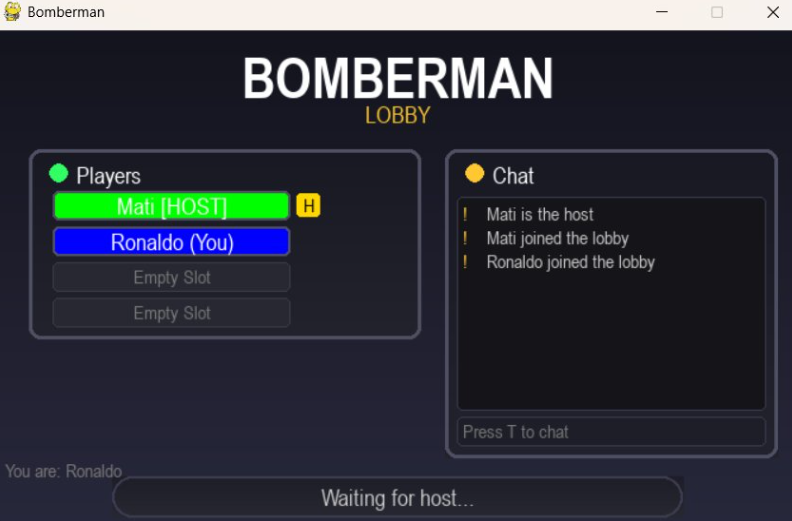
\includegraphics[width=0.75\textwidth]{figures/lobby.png}
    \caption{The lobby screen with two connected players. The host is highlighted in green.}
    \label{fig:lobby}
\end{figure}

\paragraph{Gameplay.}
Controls: \textbf{arrow keys} to move, \textbf{Space} to place a bomb.
Bombs explode after a fixed timer, destroying breakable blocks and damaging players within range.
A player loses one life per explosion hit; after three hits the player is eliminated.

\begin{figure}[H]
    \centering
    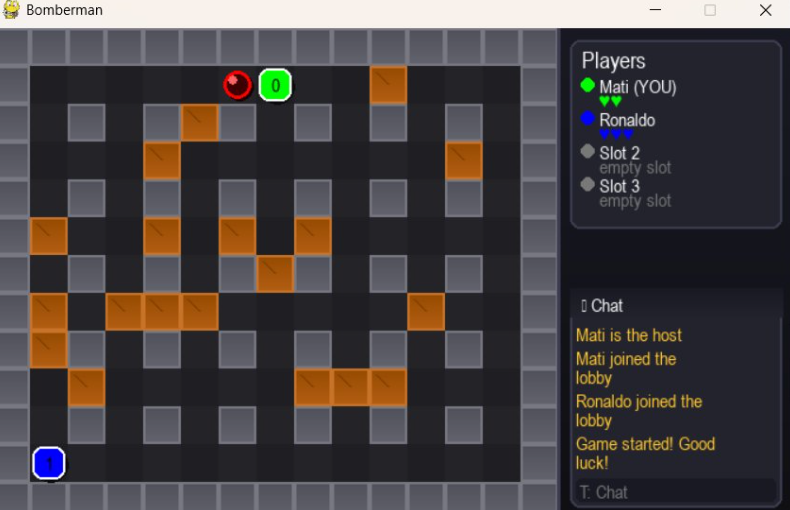
\includegraphics[width=0.75\textwidth]{figures/gameplay.png}
    \caption{The game screen during an active match. Players, breakable blocks, and the chat sidebar are visible.}
    \label{fig:gameplay}
\end{figure}

\begin{figure}[H]
    \centering
    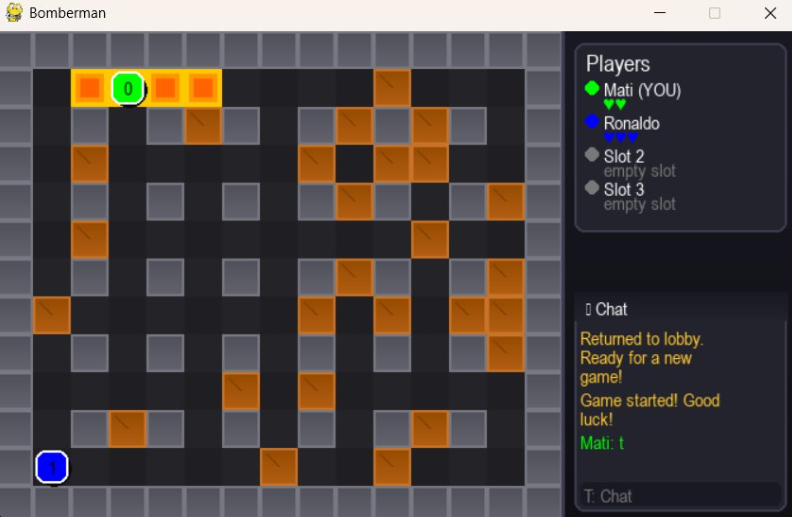
\includegraphics[width=0.75\textwidth]{figures/bomb.png}
    \caption{A bomb explosion in progress, showing the blast radius across adjacent tiles.}
    \label{fig:bomb}
\end{figure}

\paragraph{Chat.}
Press \textbf{T} to open the chat input, \textbf{Enter} to send, \textbf{Escape} to cancel.
Messages are broadcast to all connected players and spectators.

\begin{figure}[H]
    \centering
    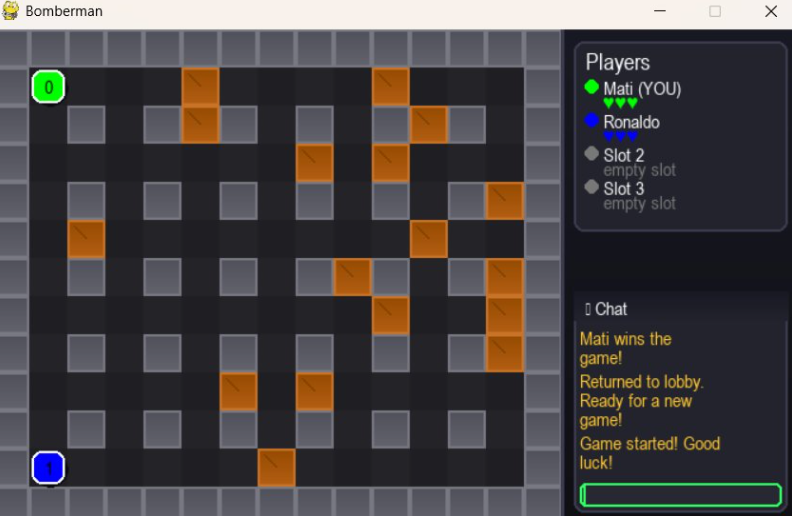
\includegraphics[width=0.75\textwidth]{figures/chat.png}
    \caption{The in-game chat input active during a match.}
    \label{fig:chat}
\end{figure}

\paragraph{End of match.}
The last surviving player wins; if all players die simultaneously, the match is a draw.
The victory screen displays the winner and a countdown before returning all clients to the lobby automatically.

\begin{figure}[H]
    \centering
    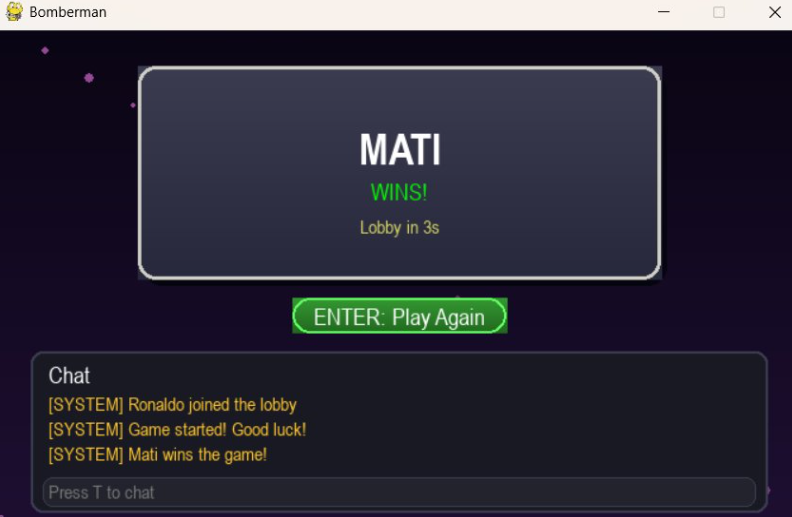
\includegraphics[width=0.75\textwidth]{figures/victory.png}
    \caption{The victory screen showing the winner and the return-to-lobby countdown.}
    \label{fig:victory}
\end{figure}

% -----------------------------------------------------------------------
\section{Self-evaluation}\label{self-evaluation}
% -----------------------------------------------------------------------

\subsection{Giovanni Rinchiuso}

My contributions span three areas: the \textbf{fault-tolerance infrastructure}, the \textbf{transparency layer}, and the \textbf{client} with its test suite.

For fault tolerance, I designed and implemented the full primary/backup stack from scratch: \texttt{FailureDetector} (heartbeat-based failure detection with a 1.5\,s timeout), \texttt{BackupServer} (state receiver, heartbeat monitor, promotion logic), \texttt{PrimaryServer} (heartbeat responder, state replication sender), and \texttt{AutoSpawner} (subprocess-based backup lifecycle management with automatic respawn on unexpected termination).
The heartbeat timeout and replication interval (100\,ms) were tuned through manual testing to balance detection speed against false positives under normal load.

The transparency layer is the TCP proxy (\texttt{fault\_tolerance/proxy\_server.py}), which hides the primary/backup topology from clients entirely.
The proxy intercepts the server's \texttt{join\_success} message to extract the \texttt{session\_id}, buffers outgoing client messages in \texttt{client\_buf} during failover, and sends a \texttt{RECONNECT} handshake to the new primary once it comes up.
A known weakness is that the proxy is itself a single point of failure: a crash severs all client connections even if the server cluster is healthy.
This is a deliberate trade-off --- unlike the primary, the proxy holds no game state, so a crash does not lose match data --- and its impact is bounded: I also implemented a client-side retry loop that re-establishes the connection every two seconds and replays the \texttt{RECONNECT} handshake, so a restarted proxy restores each player's session instead of forcing a fresh join.
It does not preserve a match in progress, since the primary observes the disconnections and resolves the victory condition immediately; bounding that would require a server-side grace period, while removing the dependency altogether would require replicating the proxy behind a virtual address.

On the client side, I built the entire Pygame application: the MVC structure (\texttt{GameController}, \texttt{GameState}, views for lobby, game, and victory), the \texttt{NetworkManager} (TCP connection, line-delimited JSON framing, background receive thread), and all graphical rendering.
I also wrote the bulk of the automated test suite: \texttt{test\_core.py},
\texttt{test\_game.py} (31 tests), \texttt{test\_controller.py} (28 tests), and
\texttt{test\_game\_service.py} (19 tests).
A limitation of the current replication design is that the primary opens a new TCP connection for every snapshot (every 100\,ms), rather than maintaining a persistent replication channel.
This is functional at the current scale but would be worth revisiting if the replication interval were reduced or the state size increased significantly.

\subsection{Gioele Santi}

My contributions are the \textbf{server game logic}, the \textbf{consistency
layer}, and the \textbf{hardening of the replication path}.

I built the authoritative game engine: map generation with destructible blocks
and safe spawn zones, bomb placement and explosion propagation (cross-shaped
blast, radius 2, with chain reactions), player lifecycle management, the
lobby/playing/victory state machine, and the spectator system. It was later
refactored so that the pure game rules in \texttt{core.py} carry no networking or
threading concern and can be unit-tested in isolation.

For consistency I implemented the \texttt{GameService} layer --- the single
component authorised to mutate game state --- protecting every public method with
a \texttt{threading.RLock} via a \texttt{@\_synchronized} decorator. Previously
the shared \texttt{State} was mutated by the game-loop thread, the accept thread
and every client handler thread with no synchronisation at all. I chose one
coarse-grained lock over per-collection locks deliberately: at 10\,Hz the
contention is negligible, while every public mutation becomes trivially atomic
and no deadlock from inconsistent lock ordering is possible. The lock must be
re-entrant because some service methods invoke others.

The replication path originally serialised state with \texttt{pickle}; since
\texttt{pickle.loads} executes arbitrary code during deserialisation, any peer
reaching the backup's state port could have achieved remote code execution. I
replaced it with a versioned JSON codec that validates the schema version and
rejects malformed snapshots instead of crashing the receiver, and covered it with
round-trip tests, since a single dropped field would silently corrupt the backup
at promotion time. I also replaced the session identifier generator --- roughly
ninety thousand brute-forceable values, enough for an attacker on the same LAN to
hijack a disconnected player's session --- with UUID4.

Finally I removed around 350 lines of dead code, which exposed a latent
\texttt{AttributeError} reachable from inside the game loop that no test covered;
I fixed it and added the missing regression test.

The main weakness in my part is that reconnection is narrower than it could be: a
client whose process exits cannot rejoin, because the \texttt{session\_id} lives
only in the client's memory and there is no server-side grace timer bounding how
long a disconnected player is retained. A transient socket drop is recovered while
enough players remain alive, but \texttt{handle\_player\_disconnect} evaluates the
victory condition immediately, so in a two-player match a single drop already ends
the round. Generalising this would require persisting the session identifier
client-side and driving an explicit expiry timer from the game loop, so that a
brief absence suspends the victory check instead of resolving it.

% -----------------------------------------------------------------------
\section{Future Works}\label{future-works}
% -----------------------------------------------------------------------

\begin{itemize}
    \item \textbf{Async I/O}: replace the thread-per-client model with \texttt{asyncio} to improve scalability.
    \item \textbf{Proxy fault tolerance}: the client-side reconnect loop already bounds
    the impact of a proxy restart, but the proxy address is statically configured, so
    the permanent loss of its host still takes the system down. Replicating the proxy
    behind a virtual address would remove that dependency.
    \item \textbf{Disconnection grace period}: suspend the victory check for a short
    window after a player disconnects, so that a transport failure --- a proxy restart
    in particular --- does not decide a match that the players could otherwise resume.
    \item \textbf{Persistent state}: write state snapshots to disk so that a complete cluster restart can recover the last known game state.
    \item Add collectable power-ups (increased bomb range, extra bomb, speed boost) to enrich gameplay.
    \item Support multiple simultaneous game rooms on the same server cluster.
    \item \textbf{Authentication}: add a simple username/password login to allow persistent scores across sessions.
    \item Automate the failover acceptance test using subprocess management and virtual network interfaces, removing the current need for manual steps.
    \item \textbf{Process lifecycle}: the backup is spawned as a child process but
    is not reaped when the primary terminates abnormally, so orphaned backups can
    survive and keep their ports bound. Placing the cluster in a process group, or
    supervising it with a dedicated launcher, would make shutdown deterministic.
\end{itemize}

\end{document}